\documentclass[12pt]{article}
\usepackage[utf8]{inputenc}
\usepackage{float}
\usepackage{amsmath}
\usepackage{amsthm}

\usepackage[hmargin=3cm,vmargin=6.0cm]{geometry}
%\topmargin=0cm
\topmargin=-2cm
\addtolength{\textheight}{6.5cm}
\addtolength{\textwidth}{2.0cm}
%\setlength{\leftmargin}{-5cm}
\setlength{\oddsidemargin}{0.0cm}
\setlength{\evensidemargin}{0.0cm}

%misc libraries goes here
\usepackage{tikz}
\usetikzlibrary{automata,positioning}


\begin{document}

\section*{Student Information } 
%Write your full name and id number between the colon and newline
%Put one empty space character after colon and before newline
Full Name :  Onur Can TIRTIR\\
Id Number :  2099380\\

% Write your answers below the section tags
\section*{Answer 1}

\subsection*{a.}
Since the claim given in the question is an \textit{if and only if} statement, we should break it into two \textit{if} directions as below. When two directions are proven, actual proof is done.

\begin{proof}
Say $e$ is an edge and $a$ and $b$ are vertices such that $a$ and $b$ are connected to each other with $e$.
\begin{enumerate}
\item{If an edge in a simple graph is a cut edge then this edge is not a part of any simple circuit in the graph.}

\textit{contradiction.} We know $e$ is a cut edge. Assume $e$ is included in a simple circuit $C$. Since $e$ is a cut edge, if we remove $e$, then we have more components in our graph than before. That means two subgraphs $A$, $B$ including $a$, $b$ respectively cannot be connected by an edge different than $e$, so we cannot complete our \textbf{simple} circuit $C$. This is because if $C$ is a simple circuit, then we cannot pass through $e$ more than once and we have no edge connecting these two subgraphs different than $e$. Hence an attempt to draw a simple circuit including $e$ will fail. Therefore our assumption is false, which is a contradiction. So we can say that if $e$ is a cut edge, then it cannot be included in a simple circuit.
\item{If an edge is not a part of any simple circuit in the graph then this edge is a cut edge.}

Since $e$ is not a part of a simple circuit, then we have no other edges between $a$ and $b$ because if we have other edges then we could construct a simple circuit. That means if we remove the edge $e$ from the graph, then $a$ and $b$ are in the different components. We know that, before the removal of $e$, they are in the same component. This tells us that $e$ is a cut edge.            
\end{enumerate}
\end{proof}

\subsection*{b.}

Consider the graph $G$.
\begin{enumerate}
\item
Assume $G$ is a connected graph. By the handshaking therom, there must be even number of vertices of odd degrees. Since it is a connected graph, then we must have at least one path from one odd degree vertice to another.
\item
Assume $G$ is a disconnected graph. Consider a connected subgraph $H$ of the graph $G$. Then the same case explained above occurs for $H$. Then, again, we must have at least one path from one odd degree vertice to another within the $H$.
\end{enumerate}

\subsection*{c.}

\begin{enumerate}
\item{\textbf{First part of the question}}\\ \\
\textbf{Initial State}\\ \\
First represent the initial state chessboard in a graph. Note that since we cannot go to the square in the middle of the chessboard, it is not needed to put a vertice representing this square. Out graph's edges will represent from which square to another we can go. $a$ represents the square left of the middle row and $b$ represents the square right of the middle row.\\

\begin{center}
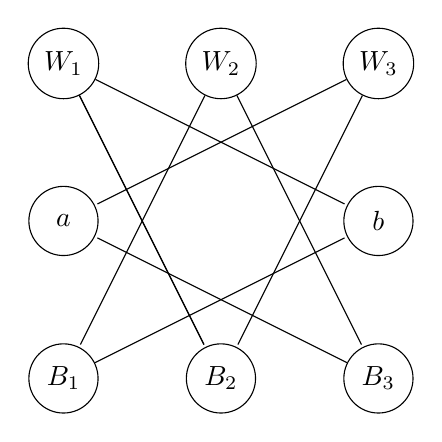
\begin{tikzpicture}[shorten >=1pt,node distance=2cm,on grid,auto]
\node[state] (W_1){$W_1$};
\node[state] (W_2) [right=of W_1] {$W_2$};
\node[state] (W_3) [right=of W_2] {$W_3$};
\node[state] (a) [below=of W_1] {$a$};
\node[state] (b) [below=of W_3] {$b$};
\node[state] (B_1) [below=of a] {$B_1$};
\node[state] (B_2) [right=of B_1] {$B_2$};
\node[state] (B_3) [right=of B_2] {$B_3$};
\path[-]
	(W_1) edge node {} (B_2)
		  edge node {} (b)
	(W_2) edge node {} (B_1)
		  edge node {} (B_3)
	(W_3) edge node {} (a)
		  edge node {} (B_2)
	(B_3) edge node {} (a)
	(W_1) edge node {} (B_2)
	(B_1) edge node {} (b) ;
\end{tikzpicture}
\end{center}

This graph is isomorphic with\\
\begin{center}
\begin{tikzpicture}[shorten >=1pt,node distance=2cm,on grid,auto]
\node[state] (W_2)  [above left=of B_3] {$W_2$};
\node[state] (B_1) [below left=of W_2] {$B_1$};
\node[state] (b) [below=of B_1] {$b$};
\node[state] (W_1) [below=of b] {$W_1$};
\node[state] (B_2) [below right=of W_1] {$B_2$};
\node[state] (W_3) [above right=of B_2] {$W_3$};
\node[state] (a) [above =of W_3] {$a$};
\node[state] (B_3) [above=of a] {$B_3$};
\path[-]
	(W_1) edge node {} (B_2)
		  edge node {} (b)
	(W_2) edge node {} (B_1)
		  edge node {} (B_3)
	(W_3) edge node {} (a)
		  edge node {} (B_2)
	(B_3) edge node {} (a)
	(W_1) edge node {} (B_2)
	(B_1) edge node {} (b) ;
\end{tikzpicture}
\end{center}

We can think of a path, ignoring $a$ and $b$ such that $W_2$, $B_3$, $W_3$, $B_2$, $W_1$, $B_1$.\\

\textbf{Final State 1}\\ \\

\begin{center}
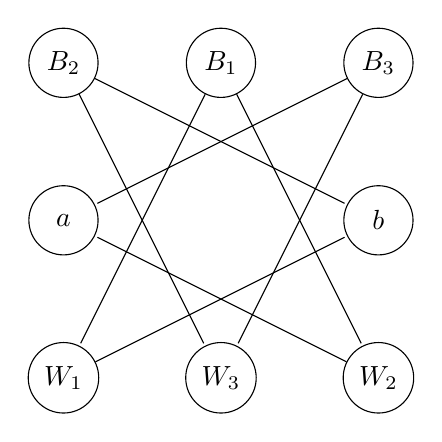
\begin{tikzpicture}[shorten >=1pt,node distance=2cm,on grid,auto]
\node[state] (B_2){$B_2$};
\node[state] (B_1) [right=of B_2] {$B_1$};
\node[state] (B_3) [right=of B_1] {$B_3$};
\node[state] (a) [below=of B_2] {$a$};
\node[state] (b) [below=of B_3] {$b$};
\node[state] (W_1) [below=of a] {$W_1$};
\node[state] (W_3) [right=of W_1] {$W_3$};
\node[state] (W_2) [right=of W_3] {$W_2$};
\path[-]
	(B_2) edge node {} (W_3)
		  edge node {} (b)
	(B_1) edge node {} (W_1)
		  edge node {} (W_2)
	(B_3) edge node {} (a)
		  edge node {} (W_3)
	(W_2) edge node {} (a)
	(W_1) edge node {} (b);
\end{tikzpicture}
\end{center}

This graph is isomorphic with\\
\begin{center}
\begin{tikzpicture}[shorten >=1pt,node distance=2cm,on grid,auto]
\node[state] (B_1)  [above left=of W_2] {$B_1$};
\node[state] (W_1) [below left=of B_1] {$W_1$};
\node[state] (b) [below=of W_1] {$b$};
\node[state] (B_2) [below=of b] {$B_2$};
\node[state] (W_3) [below right=of B_2] {$W_3$};
\node[state] (B_3) [above right=of W_3] {$B_3$};
\node[state] (a) [above =of B_3] {$a$};
\node[state] (W_2) [above=of a] {$W_2$};
\path[-]
	(B_2) edge node {} (W_3)
		  edge node {} (b)
	(B_1) edge node {} (W_1)
		  edge node {} (W_2)
	(B_3) edge node {} (a)
		  edge node {} (W_3)
	(W_2) edge node {} (a)
	(W_1) edge node {} (b);
\end{tikzpicture}
\end{center}

We can think of a path, ignoring $a$ and $b$ such that $W_2$, $B_3$, $W_3$, $B_2$, $W_1$, $B_1$. \\ \\ \\ \\ \\ \\ \\

\textbf{Final State 2}\\ \\

\begin{center}
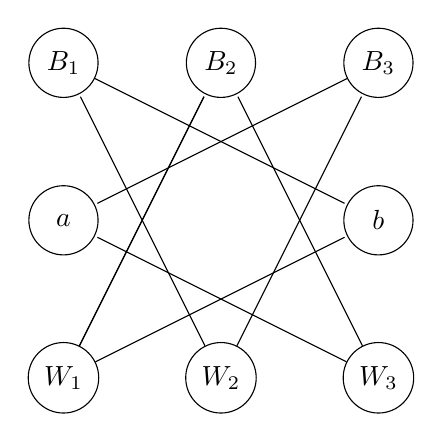
\begin{tikzpicture}[shorten >=1pt,node distance=2cm,on grid,auto]
\node[state] (B_1){$B_1$};
\node[state] (B_2) [right=of B_1] {$B_2$};
\node[state] (B_3) [right=of B_2] {$B_3$};
\node[state] (a) [below=of B_1] {$a$};
\node[state] (b) [below=of B_3] {$b$};
\node[state] (W_1) [below=of a] {$W_1$};
\node[state] (W_2) [right=of W_1] {$W_2$};
\node[state] (W_3) [right=of W_2] {$W_3$};
\path[-]
	(W_1) edge node {} (B_2)
		  edge node {} (b)
	(W_2) edge node {} (B_1)
		  edge node {} (B_3)
	(W_3) edge node {} (a)
		  edge node {} (B_2)
	(B_3) edge node {} (a)
	(W_1) edge node {} (B_2)
	(B_1) edge node {} (b) ;
\end{tikzpicture}
\end{center}

This graph is isomorphic with\\
\begin{center}
\begin{tikzpicture}[shorten >=1pt,node distance=2cm,on grid,auto]
\node[state] (B_2)  [above left=of W_3] {$B_2$};
\node[state] (W_1) [below left=of B_2] {$W_1$};
\node[state] (b) [below=of W_1] {$b$};
\node[state] (B_1) [below=of b] {$B_1$};
\node[state] (W_2) [below right=of B_1] {$W_2$};
\node[state] (B_3) [above right=of W_2] {$B_3$};
\node[state] (a) [above =of B_3] {$a$};
\node[state] (W_3) [above=of a] {$W_3$};
\path[-]
	(W_1) edge node {} (B_2)
		  edge node {} (b)
	(W_2) edge node {} (B_1)
		  edge node {} (B_3)
	(W_3) edge node {} (a)
		  edge node {} (B_2)
	(B_3) edge node {} (a)
	(W_1) edge node {} (B_2)
	(B_1) edge node {} (b) ;
\end{tikzpicture}
\end{center}

We can think of a path, ignoring $a$ and $b$ such that$B_1$, $W_1$, $B_2$, $W_3$, $B_3$, $W_2$.

Ignoring the vertices $a$ and $b$, we could find the same path in \textit{initial} and \textit{final state 1}. Note that to swap the positions of two knights, we are only allowed to move them through the initially empty squares $a$ and $b$, which means we can only shift the positions of knights once at each step. So we can easily reach from the \textit{initial state} to \textit{final state 1}.\\ \\
Also note that the paths obtained in \textit{initial state} and \textit{final state 2} are symmetric to each other.Hence we can say that even if we shift the vertices in $initial state$ graph infinitely many, we can never reach to the \textit{final state 2}. Since our only allowed move is $shifting$, there is no way to reach \textit{final state 2}.

\item{\textbf{Second part of the question}}\\ \\
In a $3\times 3$ chess board, we have $3$ to options to attempt a knight's tour.\\ \\
At any stage of knight's tour, if we are in the middle of chessboard, we cannot reach anywhere because of the shape of the move done by a knight.\\ \\
At any stage of the knight's tour, if we are in a square placed in the middle of any side, we can only reach to one of the corners. Smilarly, at any stage, if we are in one of the squares, we can only reach a square placed in the middle of any side. Hence, in such a case, we can never reach to the middle square.\\ \\
So we cannot do a knight's tour in a $3\times 3$ chessboard.

\end{enumerate}

\section*{Answer 2}
Since $A_1$ and $A_2$ have no friends in common, then the set of acquaitances $N_1$ and $N_2$ are disjoint. Take $x\in N_1$. Since $x$ and $A_2$ do not know each other, then they have $2$ friends in common by hypothesis, one of which is $A_1$, and the other one, say $y$, is from the set $N_2$ since $A_2$ cannot know any defendant from the set $N_1$. Then we can say that \textit{for every $x\in N_1$, there is a unique $y\in N_2$}. So we could construct a $1-1$ correspondance between the elements of $N_1$ and $N_2$. Then $|N_1|=|N_2|$, which means $A_1$ and $A_2$ know same number of defendants.
\section*{Answer 3}

\textit{contradiction}. Assume that there does not exist $3$ students, each from different school, that know each other. Say we have the schools $P$, $Q$ and $R$. These schools have the students $p_i$, $q_i$, $r_i$ respectively and we will construct a graph where these students are the vertices, where an edge connecting two vertices $v_1$ and $v_2$ tells us that $v_1$ and $v_2$ knows each other. Say $k$ is the maximum number of students that a student can know from a school. Suppose the student $w$ studies at the school $P$, without loss of generality, and has $k$ friends, $Q^{'}=q_1,q_2,\dots,q_k$ from the school $Q$. So $w$ must have $n+1-k$ friends, $R^{'}=r_1,r_2,\dots,r_{n+1-k}$ from the school $R$. Any student $t$ in $R^{'}$ cannot know one from $Q'$ because in that case, we have the cycles connecting $3$ vertices to each other so $t$ can know $n-k$ of the students from $R$, at most. Therefore $t$ should know $(n+1)-(n-k)=k+1$ students from $P$, which is impossible since $k+1>k$ and $k$ was the maximum number of students that can be known from a school, by a student. This is a contradiction. Hence the claim given in the quesiton is true.

\end{document}

​

